\documentclass[paper=a4, fontsize=11pt]{article} % A4 paper and 11pt font size
\usepackage[a4paper, margin=1.3in]{geometry}
% a)- Entrada y salida de texto -----

\usepackage[T1]{fontenc} % Use 8-bit encoding that has 256 glyphs
\usepackage[utf8]{inputenc}
% \usepackage[light,math]{iwona}

\usepackage{fancyhdr}
\usepackage{fancybox}
\usepackage{pseudocode}


% ---- Idioma --------

\usepackage[spanish, es-tabla]{babel} % Selecciona el español para palabras introducidas automáticamente, p.ej. "septiembre" en la fecha y especifica que se use la palabra Tabla en vez de Cuadro

% ---- Otros paquetes ----

\usepackage{amsmath,amsfonts,amsthm} % Math packages
\usepackage{graphics,graphicx, floatrow} %para incluir imágenes y notas en las imágenes
\usepackage{graphics,graphicx, float} %para incluir imágenes y colocarlas
\usepackage{enumerate}
\usepackage{subfigure}
% \makesavenoteenv{tabular}
% \makesavenoteenv{table}
% Para hacer tablas comlejas
%\usepackage{multirow}
%\usepackage{threeparttable}
\usepackage{sectsty} % Allows customizing section commands
\allsectionsfont{\centering \scshape} % Make all sections centered, the default font and small caps

\usepackage{fancyhdr} % Custom headers and footers
\usepackage[usenames, dvipsnames]{color}
\usepackage{colortbl}
% \usepackage{minted}
\usepackage{xcolor}
\usepackage{url}
\usepackage{cancel}

% \newmintedfile[mycpp]{c++}{
%     linenos,
%     numbersep=5pt,
%     gobble=0,
%     frame=lines,
%     framesep=2mm,
% }

% \newmintedfile[myc]{c}{
%     linenos,
%     numbersep=5pt,
%     gobble=0,
%     frame=lines,
%     framesep=2mm,
% }

% \newmintedfile[mypython]{python}{
%     linenos,
%     numbersep=5pt,
%     gobble=0,
%     frame=lines,
%     framesep=2mm,
% }

\usepackage{cite}

\usepackage[bookmarks=true,
    bookmarksnumbered=false, % true means bookmarks in
             % left window are numbered
    bookmarksopen=false,   % true means only level 1
             % are displayed.
    colorlinks=true,
    urlcolor=webblue,
    citecolor=webred,
    linkcolor=webblue]{hyperref}
\definecolor{webgreen}{rgb}{0, 0.5, 0} % less intense green
\definecolor{webblue}{rgb}{0, 0, 0.5}  % less intense blue
\definecolor{webred}{rgb}{0.5, 0, 0} % less intense red

%% Define a new 'leo' style for the package that will use a smaller font.
\makeatletter
\def\url@leostyle{%
  \@ifundefined{selectfont}{\def\UrlFont{\sf}}{\def\UrlFont{\small\ttfamily}}}
\makeatother
%% Now actually use the newly defined style.
\urlstyle{leo}

\pagestyle{fancyplain} % Makes all pages in the document conform to the custom headers and footers
\fancyhead{} % No page header - if you want one, create it in the same way as the footers below
\fancyfoot[L]{} % Empty left footer
\fancyfoot[C]{} % Empty center footer
\fancyfoot[R]{\thepage} % Page numbering for right footer
\renewcommand{\headrulewidth}{0pt} % Remove header underlines
\renewcommand{\footrulewidth}{0pt} % Remove footer underlines
\setlength{\headheight}{13.6pt} % Customize the height of the header

\numberwithin{equation}{section} % Number equations within sections (i.e. 1.1, 1.2, 2.1, 2.2 instead of 1, 2, 3, 4)
\numberwithin{figure}{section} % Number figures within sections (i.e. 1.1, 1.2, 2.1, 2.2 instead of 1, 2, 3, 4)
\numberwithin{table}{section} % Number tables within sections (i.e. 1.1, 1.2, 2.1, 2.2 instead of 1, 2, 3, 4)

\setlength\parindent{0pt} % Removes all indentation from paragraphs - comment this line for an assignment with lots of text

\newcommand{\horrule}[1]{\rule{\linewidth}{#1}} % Create horizontal rule command with 1 argument of height

%%%%% Para cambiar el tipo de letra en el título de la sección %%%%%%%%%%%
% \usepackage{sectsty}
% \chapterfont{\fontfamily{pag}\selectfont} %% for chapter if you want
% \sectionfont{\fontfamily{pag}\selectfont}
% \subsectionfont{\fontfamily{pag}\selectfont}
% \subsubsectionfont{\fontfamily{pag}\selectfont}

%----------------------------------------------------------------------------------------
% TÍTULO Y DATOS DEL ALUMNO
%----------------------------------------------------------------------------------------

\title{
\normalfont \normalsize
\textsc{{\bf Redes y Sistemas Complejos (2016-2017)} \\ Grado en Ingeniería Informática \\ Universidad de Granada} \\ [25pt] % Your university, school and/or department name(s)
\horrule{0.5pt} \\[0.4cm] % Thin top horizontal rule
\huge Memoria Práctica 2-5\\ Modelos de NetLogo: Redes Aleatorias\\% The assignment title
\horrule{2pt} \\[0.5cm] % Thick bottom horizontal rule
}

\author{Braulio Vargas López\\DNI: 20079894C\\Correo: brauliovarlop@correo.ugr.es} % Nombre y apellidos

\date{\normalsize\today} % Incluye la fecha actual

%----------------------------------------------------------------------------------------
% DOCUMENTO
%----------------------------------------------------------------------------------------

\begin{document}

\maketitle % Muestra el Título
\pagenumbering{gobble}
\newpage %inserta un salto de página

\tableofcontents % para generar el índice de contenidos

\pagenumbering{arabic}
\section{Ejercicio 1}
\textit{Si el tamaño de una red de Erdös-Renyi se incrementa 100 cien veces (es decir, de 100 a 10000 nodos), ¿cómo cambiará la media del camino más corto?
    \begin{enumerate}[a)]
        \item Será 100 veces más largo a lo más.
        \item Será 10 veces más largo a lo más.
        \item Será el doble de largo a lo más.
        \item Permanecerá igual.
        \item Será la mitad de largo a lo más.
    \end{enumerate}
}

Para resolver esta pregunta, he realizado dos simulaciones en NetLogo con el modelo ER. Una para una red de 10 nodos, y otra para una red de 1000. En la \hyperref[imej1]{Figura \ref{imej1}} se pueden ver los resultados para ambas simulaciones:

\begin{figure}[H]
    \centering
    \mbox{
        \subfigure[Resultados para la simulación con la red de tamaño 10.] {
            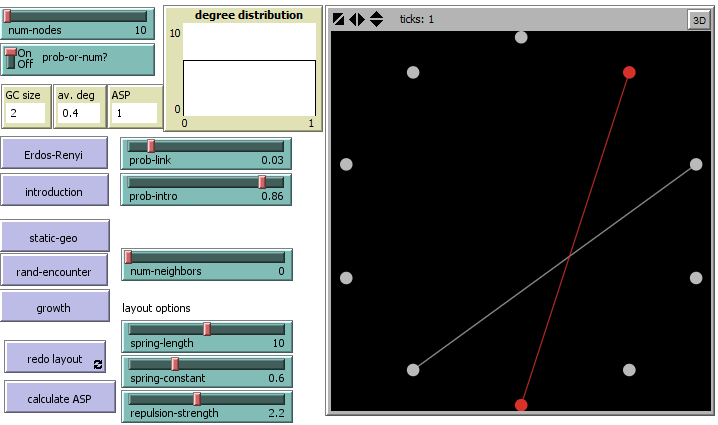
\includegraphics[width=0.5\textwidth]{img/im1}
            \label{im1}
        }
        \qquad
        \subfigure[Resultados para la simulación con la red de tamaño 1000.] {
            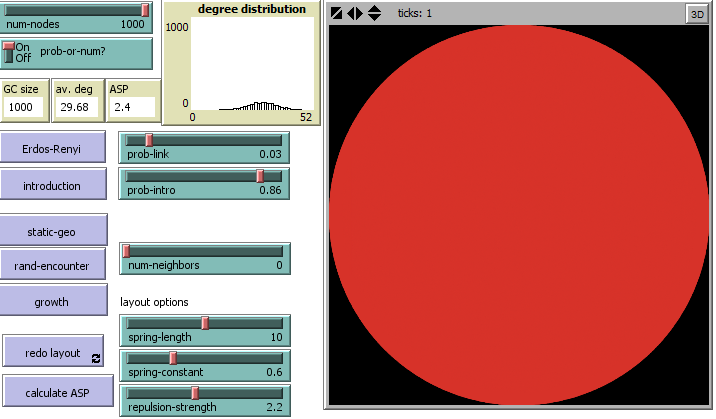
\includegraphics[width=0.5\textwidth]{img/im2}
            \label{im2}
        }
    }
    \caption{Momentos de la simulación.}
    \label{imej1}
\end{figure}

Si comparamos las distancias medias de los caminos más cortos tenemos que $\frac{2.4}{1} = 2.4 \approx 2$. Es por esto por lo que la opción correcta es la \textbf{opción C}.

\section{Ejercicio 2}
\textit{En relación con el modelo ER, el modelo introductorio 
\begin{enumerate}[a)]
    \item Tiene más ejes.
    \item Tienes más cliques.
    \item Un camino mínimo medio más largo.
    \item Un grado más irregular.
    \item Una componente gigante más pequeña con valores bajos de $p$.
\end{enumerate}
}

Para resolver esto, vamos a hacer una serie de simulaciones para ir comprobando los distintos puntos.

En la \hyperref[imej2]{Figura \ref{imej2}}, podemos ver los resultados de una primera simulación para cada uno de los models. 

\begin{figure}[H]
    \centering
    \mbox{
        \subfigure[Resultados para la simulación con \textit{introduction}.] {
            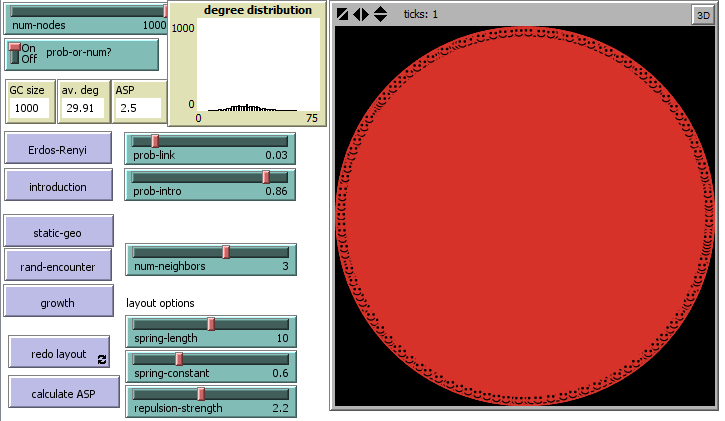
\includegraphics[width=0.5\textwidth]{img/im3}
            \label{im3}
        }
        \qquad
        \subfigure[Resultados para la simulación con \textit{ER}.] {
            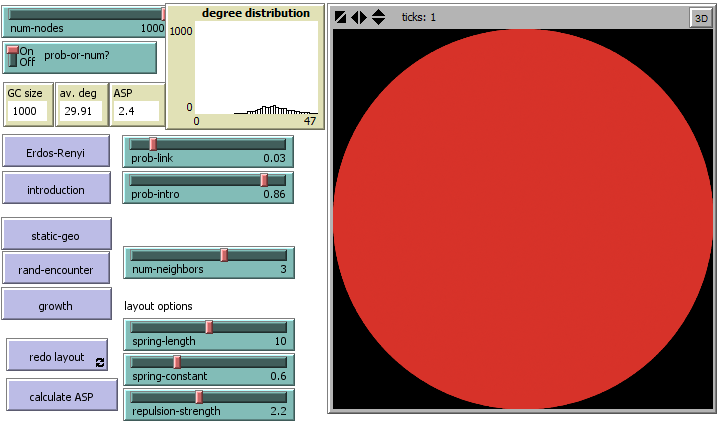
\includegraphics[width=0.5\textwidth]{img/im4}
            \label{im4}
        }
    }
    \caption{Momentos de la simulación.}
    \label{imej2}
\end{figure}

En ella podemos ver varias cosas. Una de ellas es que en la \hyperref[im3]{Figura \ref{im3}} podemos ver la distribución de grados del modelo \textit{introduction} es mucho más amplia que la distribución de grados que podemos ver en la \hyperref[im4]{Figura \ref{im4}}, además de ser un poco más irregular que la del modelo ER. Además, la longitud media del camino mínimo en el modelo \textit{introduction} es mayor que en el modelo \textit{ER}.

\begin{figure}[H]
    \centering
    \mbox{
        \subfigure[Resultados para la simulación con \textit{introduction}.] {
            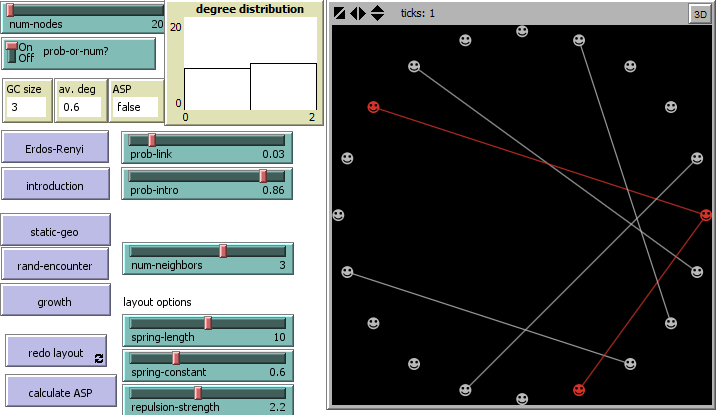
\includegraphics[width=0.5\textwidth]{img/im5}
            \label{im5}
        }
        \qquad
        \subfigure[Resultados para la simulación con \textit{ER}.] {
            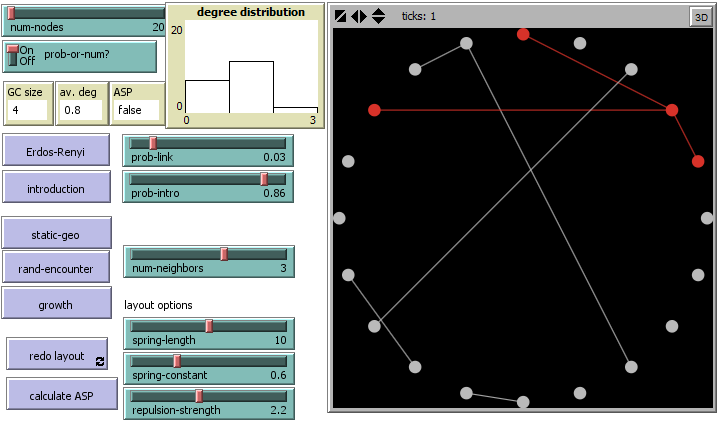
\includegraphics[width=0.5\textwidth]{img/im6}
            \label{im6}
        }
    }
    \caption{Momentos de la simulación.}
    \label{imej3}
\end{figure}

En la \hyperref[imej3]{Figura \ref{imej3}} podemos ver cómo el número de aristas es ligeramente menor en el modelo \textit{introduction} (\hyperref[im5]{Figura \ref{im5}}) al del modelo \textit{ER} (\hyperref[im6]{Figura \ref{im6}}). Esto también lo podemos ver reflejado en el grado medio de cada uno de los modelos. 

\begin{figure}[H]
    \centering
    \mbox{
        \subfigure[Resultados para la simulación con \textit{introduction}.] {
            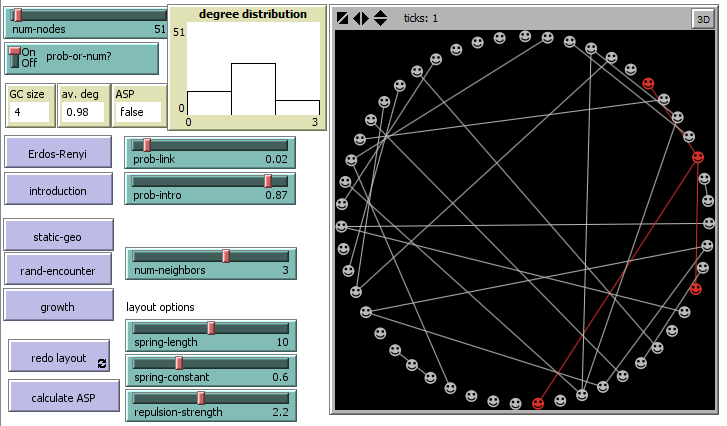
\includegraphics[width=0.5\textwidth]{img/im7}
            \label{im7}
        }
        \qquad
        \subfigure[Resultados para la simulación con \textit{ER}.] {
            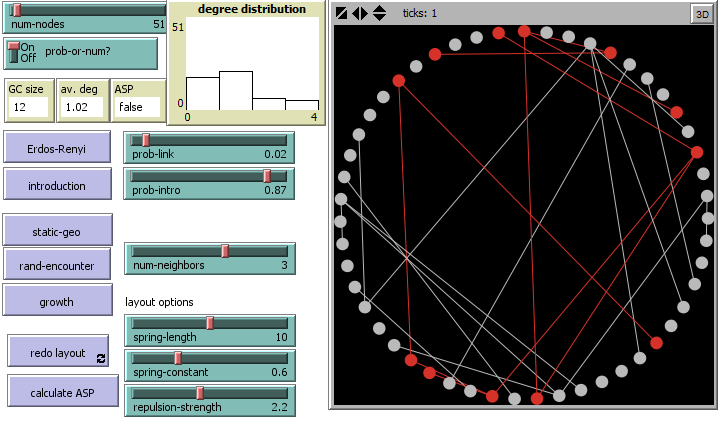
\includegraphics[width=0.5\textwidth]{img/im8}
            \label{im8}
        }
    }
    \caption{Momentos de la simulación.}
    \label{imej4}
\end{figure}

En la \hyperref[imej4]{Figura \ref{imej4}} podemos ver cómo para valores pequeños de $p$, la componente gigante del modelo \textit{introduction} (\hyperref[im7]{Figura \ref{im7}}) es más pequeña que la del modelo \textit{ER} (\hyperref[im8]{Figura \ref{im8}}). También podemos ver cómo el número de cliques o triángulos es mayor en el modelo \textit{introduction} que en el modelo \textit{ER}.

\section{Ejercicio 3}
\textit{En relación con el modelo ER, el modelo estático geográfico tiene:
\begin{enumerate}[a)]
    \item Un camino mínimo medio más largo.
    \item Un camino mínimo medio más corto.
    \item Una distribución de grados más acotada.
    \item Una distribución de grados más amplia.
    \item Una componente gigante más pequeña con menor número de vecinos.
    \item Una componente gigante más grande con menor número de vecinos.
\end{enumerate}
}

Al igual que en apartados anteriores, para resolver el ejercicio haremos una comparativa entre ambos modelos realizando varias simulaciones. Pero en este caso, tenemos que poner el flag \textit{prob-or-num} en \textbf{\textit{off}} para poder comparar ambos modelos.

\begin{figure}[H]
    \centering
    \mbox{
        \subfigure[Resultados para la simulación con \textit{static-geo}.] {
            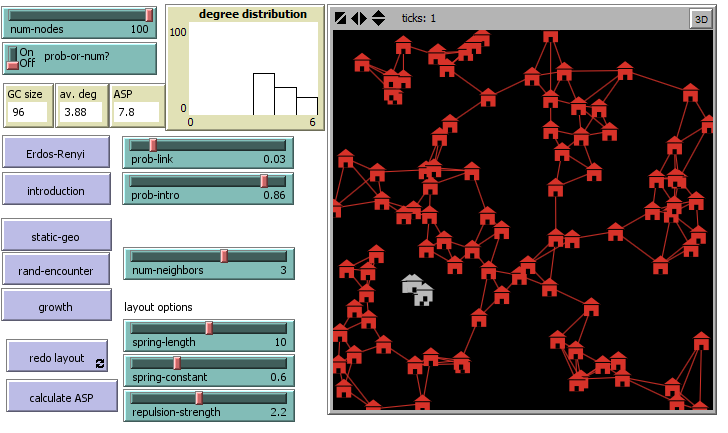
\includegraphics[width=0.5\textwidth]{img/im9}
            \label{im9}
        }
        \qquad
        \subfigure[Resultados para la simulación con \textit{ER}.] {
            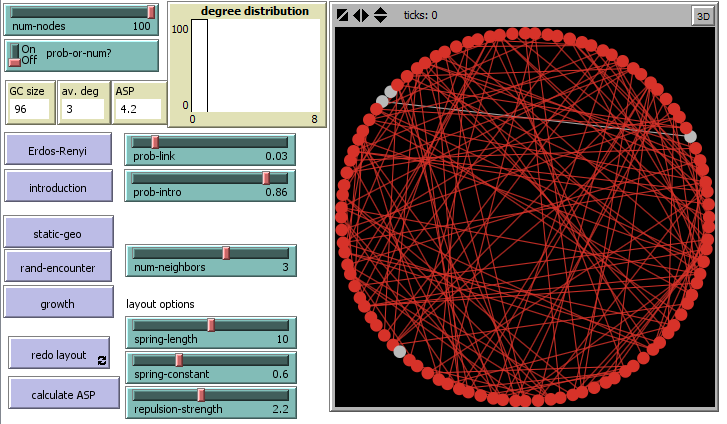
\includegraphics[width=0.5\textwidth]{img/im10}
            \label{im10}
        }
    }
    \caption{Momentos de la simulación.}
    \label{imej5}
\end{figure}

En la \hyperref[imej5]{Figura \ref{imej5}} podemos ver cómo la longitud media del camino mínimo es más larga en el modelo \textit{static-geo} que en el modelo \textit{ER} y que la distribución de grados es más amplia que en el modelo \textit{ER}. Para ver el tamapño de la componente gigante, tenemos que ver la simulación de la \hyperref[imej6]{Figura \ref*{imej6}}.

\begin{figure}[H]
    \centering
    \mbox{
        \subfigure[Resultados para la simulación con \textit{static-geo}.] {
            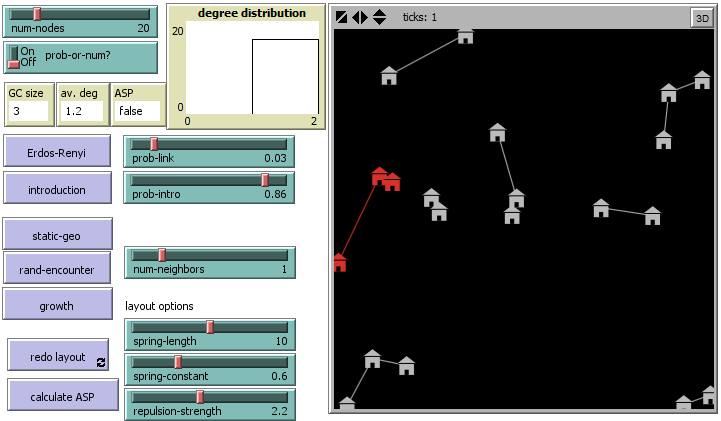
\includegraphics[width=0.5\textwidth]{img/im11}
            \label{im11}
        }
        \qquad
        \subfigure[Resultados para la simulación con \textit{ER}.] {
            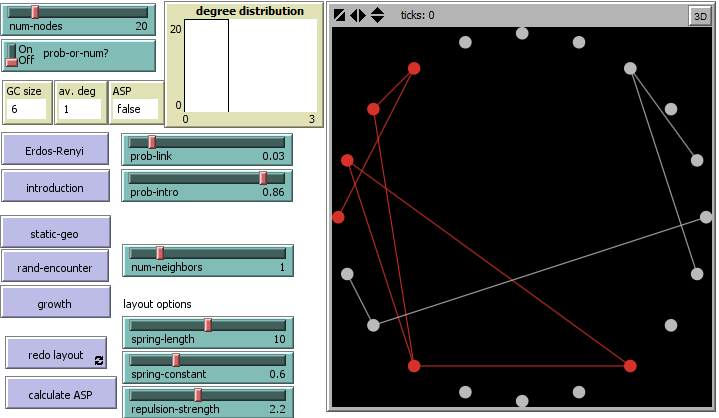
\includegraphics[width=0.5\textwidth]{img/im12}
            \label{im12}
        }
    }
    \caption{Momentos de la simulación.}
    \label{imej6}
\end{figure}

En esta imagen podemos ver claramente como la componente gigante con un menor número de vecinos es mucho menor en el modelo \textit{static-geo} (\hyperref[im11]{Figura \ref*{im11}}) que en el modelo \textit{ER} (\hyperref[im12]{Figura \ref*{im12}}).

\section{Ejercicio 4}
\textit{En relación con el modelo ER, el modelo de encuentros aleatorios tiene:
\begin{enumerate}[a)]
    \item Un mayor número de triángulos.
    \item Un menor número de triángulos.
    \item Una componente gigante menor con un menor número de vecinos.
    \item Una componente gigante mayor con un menor número de vecinos.
\end{enumerate}
}

En este caso, volvemos a generar simulaciones para ambos modelos, con el fin de compararlos y obtener las respuestas a la pregunta. Para responer al número de triángulos, podemos consultar la \hyperref[imej7]{Figura \ref*{imej7}}.

\begin{figure}[H]
    \centering
    \mbox{
        \subfigure[Resultados para la simulación con \textit{random-encounter}.] {
            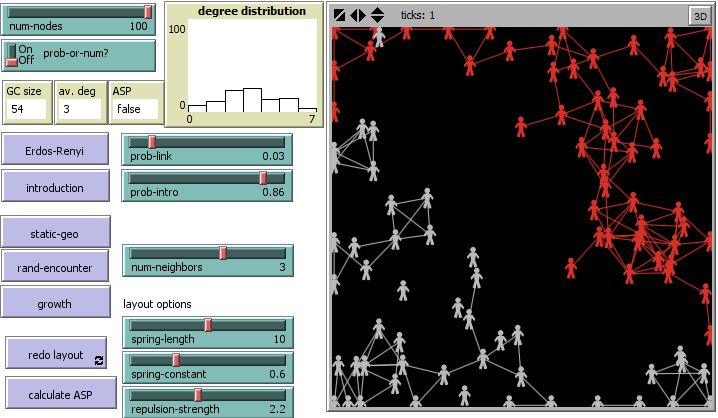
\includegraphics[width=0.5\textwidth]{img/im14}
            \label{im14}
        }
        \qquad
        \subfigure[Resultados para la simulación con \textit{ER}.] {
            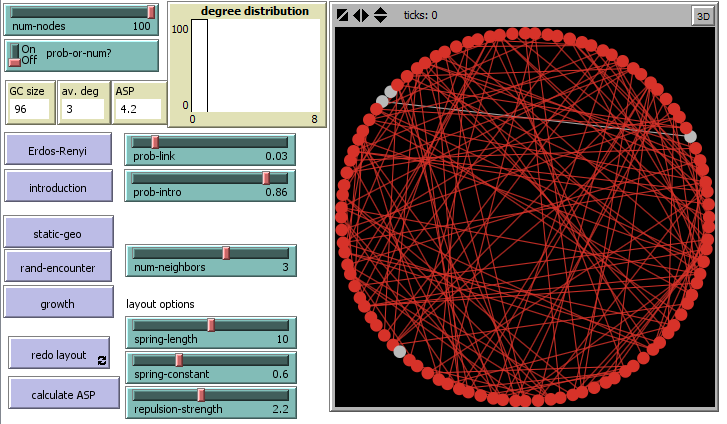
\includegraphics[width=0.5\textwidth]{img/im10}
            \label{im101}
        }
    }
    \caption{Momentos de la simulación.}
    \label{imej7}
\end{figure}

En la \hyperref[imej7]{Figura \ref*{imej7}}, podemos ver cómo el número de triángulos en el modelo \textit{random-encounter} es mayor que en el modelo \textit{ER}. El layout de NetLogo permite ver fácilmente la formación de triángulos en la red, y como se puede ver en la \hyperref[im14]{Figura \ref*{im14}}, el número de triángulo ses mayor que en la \hyperref[im101]{Figura \ref*{im101}}.

En el caso del tamaño de la componente gigante, podemos ver la \hyperref[imej8]{Figura \ref*{imej8}}, en la que podemos ver como para un menor número de vecinos, el tamaño de la componente gigante es mucho menor en el modelo \textit{random-encounter} que en el modelo \textit{ER}.

\begin{figure}[H]
    \centering
    \mbox{
        \subfigure[Resultados para la simulación con \textit{random-encounter}.] {
            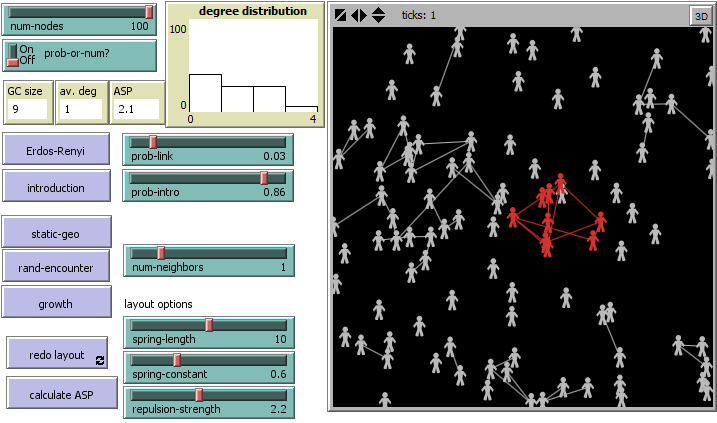
\includegraphics[width=0.5\textwidth]{img/im13}
            \label{im13}
        }
        \qquad
        \subfigure[Resultados para la simulación con \textit{ER}.] {
            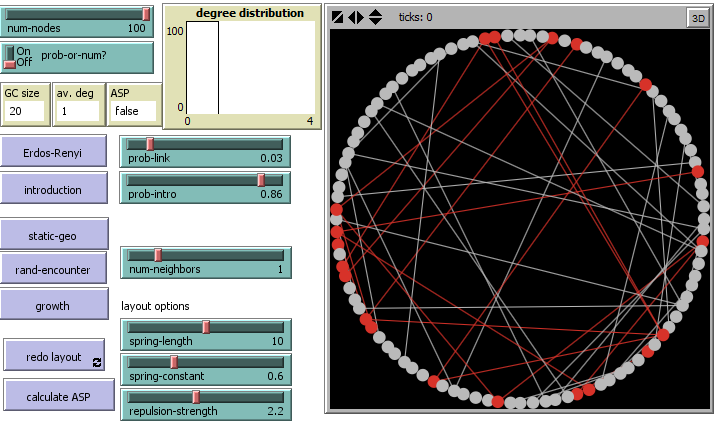
\includegraphics[width=0.5\textwidth]{img/im17}
            \label{im17}
        }
    }
    \caption{Momentos de la simulación.}
    \label{imej8}
\end{figure}

\section{Ejercicio 5}
\textit{En relación con el modelo ER, el modelo de crecimiento tiene:
\begin{enumerate}[a)]
    \item Más hubs.
    \item Menos hubs.
    \item Una componente gigante menor con un menor número de vecinos.
    \item Una componente gigante mayor con un menor número de vecinos.
\end{enumerate}
}

Para comprobar qué modelo presenta más hubs, podemos ver ambos modelos en la \hyperref[imej9]{Figura \ref*{imej9}}, donde podemos ver que el modelo \textit{growth} presenta un mayor número de hubs que el modelo \textit{ER}.

\begin{figure}[H]
    \centering
    \mbox{
        \subfigure[Resultados para la simulación con \textit{growth}.] {
            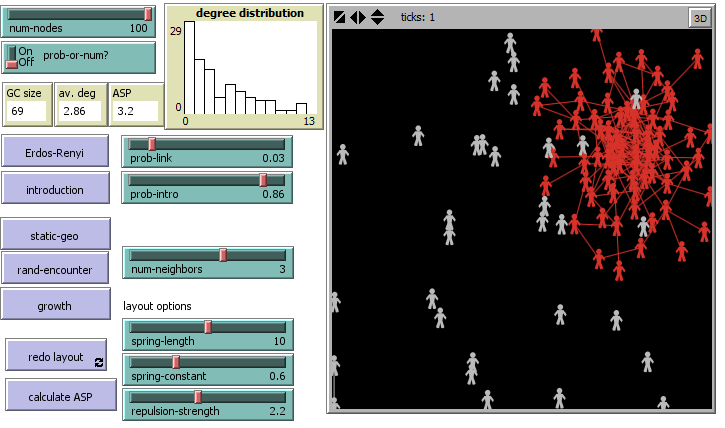
\includegraphics[width=0.5\textwidth]{img/im15}
            \label{im15}
        }
        \qquad
        \subfigure[Resultados para la simulación con \textit{ER}.] {
            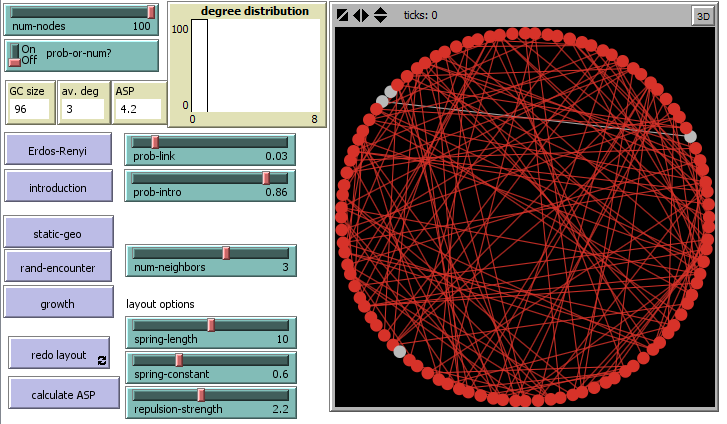
\includegraphics[width=0.5\textwidth]{img/im10}
            \label{im102}
        }
    }
    \caption{Momentos de la simulación.}
    \label{imej9}
\end{figure}

Y, en el caso del tamaño de la componente gigante, también presenta el modelo \textit{growth} una componente mucho mayor que el modelo \textit{ER} cuando presenta un pequeño número de vecinos, tal y como se puede comprobat en la \hyperref[imej10]{Figura \ref*{imej10}}.

\begin{figure}[H]
    \centering
    \mbox{
        \subfigure[Resultados para la simulación con \textit{growth}.] {
            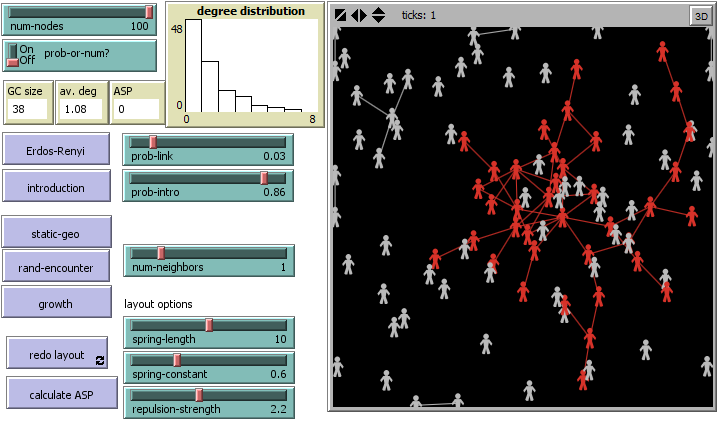
\includegraphics[width=0.5\textwidth]{img/im16}
            \label{im16}
        }
        \qquad
        \subfigure[Resultados para la simulación con \textit{ER}.] {
            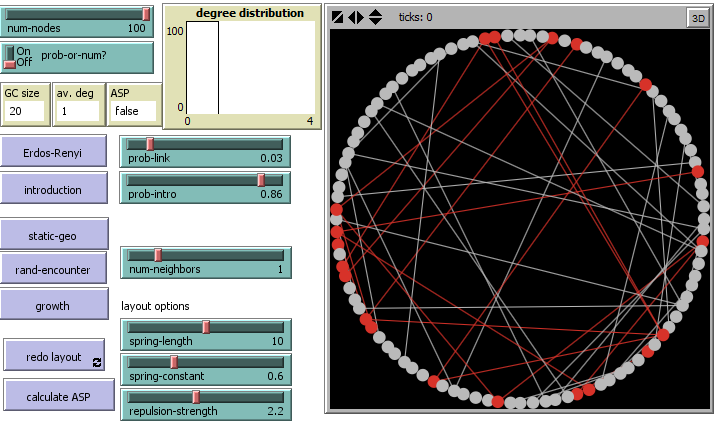
\includegraphics[width=0.5\textwidth]{img/im17}
            \label{im17}
        }
    }
    \caption{Momentos de la simulación.}
    \label{imej10}
\end{figure}

\end{document}
